 
\chapter{Conditions and sub-boxes}
  
In this section we expand on some topics mentioned briefly in
Section 1 %TODO: chxref
.  As such, it would be useful to look again at
Definitions \ref{GMT 1.8}, \ref{GMT 1.12}, and \ref{GMT 1.22}, and Remark \ref{GMT 1.9}),
where ${\mathcal P}$, ${\mathcal T}$ and their partners (under exponentiation)
${\mathcal W}$, ${\mathcal S}$ are introduced, and at
Definition \ref{GMT 1.18}
 where the notion of a killerword is introduced (the
definition is phrased in terms of ${\mathcal P}$, but the definition also makes sense for ${\mathcal W}$).  Note that working with
the region
${\mathcal P}$ is intuitively appealing, but working with the box ${\mathcal W}$ is vastly superior computationally (see
Remark \ref{GMT 1.21}
).

Theorem \ref{GMT 0.2},
hence
Theorem \ref{GMT 0.1}, follows from
Propositions \ref{GMT 1.28},
	(CHECKTHIS ref{GMT 2.8}, ref{GMT 3.1}, and ref{GMT 3.2}).  %TODO: xref to cut
  The computational aspects of the proofs of each of these propositions are similar.  We will focus on
Proposition \ref{GMT 1.28}
 here.
Its proof   amounts to decomposing 
 ${\mathcal W}$ into a collection of sub-boxes of two types:
\begin{itemize}
\item[1)]   The 11 sub-boxes which comprise the 
exceptional boxes $X_0, X_1, \ldots, X_6.$ 

\item[2)]   Sub-boxes each of which has an associated {\textit condition} that will describe how to kill that entire sub-box,
perhaps with the help of a killerword.  To {\textit kill} a sub-box means to show that 
${\mathcal S} - \bigcup_{n = 0,\dots, 6} X_n$ has no point in the sub-box. 
\end{itemize}
\noindent The set-up for efficiently describing these sub-boxes will be given in Construction \ref{GMT 5.3}. 
 

We now list the conditions used to kill the nonexceptional sub-boxes.  There are two types of conditions: the trivial and
the interesting.  The trivial conditions kill sub-boxes in ${\mathcal W}$ since the sub-boxes in question miss 
$\exp({\mathcal P}).$  The interesting conditions are where the real work is done, and they require a killerword in $f, w,
f^{-1}, w^{-1}$ to work their magic (see
Remark \ref{GMT 1.17}).

To be consistent with the computer program {\textit verify} we use the following notation: $L^{\prime} = z_0 + i z_3$,
$D^{\prime} = z_1 + i z_4,$ and $R^{\prime} = z_2 + i z_5.$  Here $(L^{\prime}, D^{\prime}, R^{\prime}) \in {\mathcal W}$ and
$L^{\prime} = \exp(L) = \exp(l+it),\   D^{\prime} = \exp(D) = \exp(d+ib),\  
R^{\prime} = \exp(R) = \exp(r+ia).$
\vglue10pt
\begin{the trivial conditions}  \label{GMT 5.1}
{\textit Condition} `s' ({\textit short}):  Tests that all points in the sub-box have $|z_0 + i z_3| < 1.10274.$  This ensures that  
$$\exp(l) = |\exp(L)| = |L^{\prime}| = |z_0 + i z_3| < 1.10274 < \exp(0.0978),$$  and
Definition \ref{GMT 1.12}
 tells us that we are
outside of $\exp({\mathcal P}).$
\vglue6pt
{\textit Condition} `l' ({\textit long}): Tests that all points in the sub-box have $|z_0 + i z_3| > 3.63201.$  This ensures that  
$$\exp(l) = |\exp(L)| = |L^{\prime}| = |z_0 + i z_3| > 3.63201 > \exp(1.289785)$$ and we are outside of $\exp({\mathcal P}).$  
\vglue6pt
{\textit Condition} `n' ({\textit near}): Tests that all points in the sub-box have $|z_1 + i z_4| < 1.$  This ensures that 
$$\exp(d) = |\exp(D)| = |D^{\prime}| = |z_1 + i z_4| <1= \exp(0)$$ and we are outside of $\exp({\mathcal P}).$
\vglue6pt
{\textit Condition} `f' ({\textit far}): Tests that all points in the sub-box have $|z_1 + i z_4| > 3.$  This ensures that 
$$\exp(d) = |\exp(D)| = |D^{\prime}| = |z_1 + i z_4|  > 3= \exp(\ln 3)$$ and we are outside of $\exp({\mathcal P}).$  
%\eject
\vskip 8pt
{\textit Condition} `w' ({\textit whirle  big}): Tests that all points in the sub-box have $|z_2 + i z_5|^2 > |z_0 + i z_3| $  This
ensures that $$\exp(r) = |\exp(R)| = |R^{\prime}| = |z_2 + i z_5|  > \sqrt{|z_0 + i z_3|} =  \sqrt {\exp(l)} = \exp(l/2)$$ and
we are outside of $\exp({\mathcal P}).$  
\vglue6pt
{\textit Condition} `W' ({\textit whirle  small}): Tests that all points in the sub-box have $|z_2 + i z_5| < 1. $  This ensures that
$$\exp(r) = |\exp(R)| = |R^{\prime}| = |z_2 + i z_5|  < 1 = \exp(0)$$ and we are outside of $\exp({\mathcal P}).$\end{the trivial conditions}

\vglue12pt
\begin{the interesting conditions}\label{GMT 5.2}
\vglue6pt
{\textit Condition}  `L': This condition comes equipped with a killerword $k$ in $f, w, f^{-1}, w^{-1},$ and tests that all
points in the sub-box have $|\exp({\textrm length}(k))| <  |L^{\prime}| = |\exp(L)|,$ where ${\textrm length}(k)$ means the length
of the isometry determined by $k.$   This, of course, contradicts the fact that $L$ is the length of the shortest geodesic.

It is easy to carry out the test $|\exp({\textrm length}(k))| <  |L^{\prime}|$ because
Lemma \ref{GMT 1.25} a) can be used.
Note that in {\textit verify} the function which computes $\exp({\textrm length})$ is called {\textit length}.  

Of course, Condition `L' also checks that the isometry corresponding to the word $k$ is not the identity.
\vglue6pt
{\textit Condition}   `O':   This condition comes equipped with a killerword 
$k$ in $f, w, f^{-1}, w^{-1},$ and tests that all points in the sub-box have 
$$|\exp({\textrm distance}(k(B_{(0,\infty)}),
B_{(0,\infty)}))| <  |D^{\prime}| = |\exp(D)|.$$    (Recall that 
$B_{(0;\infty)}$ denotes the oriented geodesic $\{(0,0,z): 0< z < \infty \}$,
with negative endpoint $(0,0,0).$)
This, of course, contradicts the ``nearest" condition.

It is easy to carry out the test $|\exp({\textrm distance}(k(B_{(0,\infty)}), B_{(0,\infty)}))| <  |D^{\prime}|$ because
Lemma \ref{GMT 1.25} b) can be used. Note that in {\textit verify} the function which computes the quantity
$$\exp({\textrm distance}(k(B_{(0,\infty)}), B_{(0,\infty)}))$$ is called {\textit orthodist}.  

Also, Condition `O' checks that the isometry corresponding to the word $k$ does not take the axis of $f$ to itself.
\vglue6pt
{\textit Condition}   `2':  This is just the `L' condition without the ``not-the-identity" check, but with the additional
proviso that the killerword $k$ is of the form $f^p w^q.$ This ensures that $k$ is not the identity, because for $k$ to be
the identity $f$ and $w$ would have to have the same axis, which contradicts the fact that $d$ can be taken to be
greater than or equal to $l/4.$
%\eject
\vskip 8pt
{\textit Condition}  `conjugate':  There is one other condition that is used to eliminate points in ${\mathcal W}.$  Following
Definition \ref{GMT 1.12}
 (and 
Lemma \ref{GMT 1.13}
) we eliminate all boxes with $0 < t \le \pi.$  Of course, after exponentiating $L = l+it,$
this corresponds to eliminating all boxes with $z_3 > 0.$ Specifically, we toss all sub-boxes of ${\mathcal W}$ whose fourth
entry is a 1. This condition does not appear in {\textit verify} because it is applied ``outside" of these
programs, as described in Construction \ref{GMT 5.3}.\end{the interesting conditions}
\vglue6pt
\begin{construction} \label{GMT 5.3}: 
We now give the method for describing the roughly 930 million sub-boxes that the initial box ${\mathcal W}$ is subdivided into.

All sub-boxes are obtained by subdivision of a previous sub-box along a real
hyper-plane midway between parallel faces of the sub-box before
subdivision.  Of course, these midway planes are of the form $x_i = $ a
constant.   We use $0$'s and $1$'s to describe which half of a subdivided
sub-box to take ($0$ corresponds to lesser $x_i$ values).  For example, 0
describes 
the sub-box $${\mathcal W} \cap \{(x_0,x_1,x_2,x_3,x_4,x_5): x_0 \le 0 \},$$ 
$010$ describes the sub-box 
$$W \cap \{(x_0,x_1,x_2,x_3, x_4,x_5) : x_0 \le 0,\ x_1 \ge 0,\ x_2 \le 0 \},$$
and so on.

In this way, we get a one-to-one correspondence
between strings and sub-boxes.
If $s$ is a string of $0$'s and $1$'s, then let $Z(s)$ denote
the sub-box corresponding to $s$.
The range of values for the $i^{\mathrm th}$ coordinate in the sub-box $Z(s)$ is related
to the binary fraction $0.s_{i}s_{i+6}\ldots s_{i+6k}$.
The two sub-boxes gotten from
subdividing $Z(s)$ are $Z(s0)$ and $Z(s1)$.

The directions of subdivision cycle among the various coordinate axes:
the $n^{\mathrm th}$ subdivision is across the $(n \bmod 6)^{\mathrm th}$ axis.
The dimensions of the top-level box ${\mathcal W}$ were chosen so that subdivision
is always done across the longest dimension of the box,
and so that all of the sub-boxes are similar.  
The dimensions of ${\mathcal W}$ have the beneficial effect of making the sub-boxes as ``round" as possible, hence making the Taylor approximation calculations efficient and fast.
This explains the factor of $2^{(5-i)/6}$ in Definition 
\ref{GMT 1.22}

To kill a sub-box $Z(s)$, the checker program has two (recursive) options:
use a condition and, if necessary, an associated killerword  to kill $Z(s)$ directly, or first kill $Z(s0)$ and then kill $Z(s1)$.
At this point, it may seem as if the second option is not necessary,
because surely a condition which kills two halves also kills the whole.
The answer to this has been hinted at in 
Remarks \ref{GMT 1.17} and \ref{GMT 1.35}
 where
it is noted that our evaluation of a function arising
from a killerword  is via first-order Taylor
approximation, complete with remainder/error term.
(Note that the remainder/error term incorporates bounds on
both the theoretical error arising from using a first-order Taylor
approximation to approximate a function, and the accumulated
round-off error; see 
	Chapters (CHECKTHIS: FIXME(6, 7,  and 8).)  %TODO: chxref
Even if a killerword could theoretically kill off a sub-box,
it is quite possible that our
first-order Taylor approximation approach would not be
able to prove this 
because its remainder/error term is too large.
However, if we subdivide the sub-box, then the first-order
Taylor approximations on the two halves should be more accurate.  
Thus,
we want to have the recursive subdivision option at our
disposal.
Note that because the checker program does in fact do such 
recursive subdivisions, the actual number of sub-boxes in the
ultimate subdivision is larger (perhaps substantially larger)
than the 930 million sub-boxes of the initial data tree.

It is also possible that the checker program will employ
neither of the two options described in the previous
paragraph, and will instead employ  
a third option: do not kill $Z(s)$, and instead
mark $s$ as omitted.
Any omitted sub-boxes are checked with another instance
of the checker program,
unless the sub-box is one of the 11 exceptional
sub-boxes (which produce the seven exceptional boxes after joining abutters).
Note that according to the definition of ``kill" given at the beginning of this section, the exceptional boxes are
automatically killed.   

Thus, a typical output from {\textit verify} would be 
\begin{eqnarray*}
&&{\textrm verified} 000000111101111111 \\
&&\qquad\qquad\quad- 
\{ 0000001111011111110 \ \ 000000111101111111110 \} .
\end{eqnarray*}
which means that the sub-box $Z(000000111101111111)$ was killed except for its sub-boxes
$Z(0000001111011111110)$  and $Z(000000111101111111110).$  The output 
\begin{eqnarray*}
&&{\textrm verified} 0000001111011111110 - \{\ \}.\\
\noalign{\noindent and}
&&{\textrm verified} 000000111101111111110 - \{\ \}.
\end{eqnarray*} shows that these sub-boxes were subsequently killed as well, and thus the entire sub-box
$Z(000000111101111111)$ has been killed. 


Instead of immediately working on killing the top-level box, we subdivide in the six co-ordinate directions to get the 64 sub-boxes $$Z(000000),Z(000001),Z(000010),Z(000011),\ldots, Z(111111).$$ 
\noindent We then throw out
the ones with fourth co-ordinate equal to 1 (see condition `conjugate'), leaving  the 32 sub-boxes
$$Z(000000),Z(000001),Z(000010),Z(000011),\ldots, Z(111011).$$  \noindent We then use {\textit verify} to kill these.
%\eject
\vskip 8pt
The choices in {\textit verify} are made for it by a sequence
of integers given as input.  The sequence of integers containing the directions for killing $Z(000000)$ is contained in the file data/000000 (actually, data/000000.d).
In such a sequence, 
$0$ tells {\textit verify} to subdivide the present box (by $x_i = c$),  to position itself on the ``left-hand" box ($x_i \le c$)
created by that subdivision, and to read in the next integer in the sequence. A  positive integer $n$ tells {\textit verify} to
kill directly the sub-box it is positioned at, using the condition (and killerword, if necessary) on line $n$ in the
``conditionlist" file,  and then to position itself at the ``next" natural sub-box.  Now,
$-1$ tells {\textit verify} to omit the sub-box, and mark it as skipped
(the sequence of integers used in killing the skipped box $Z(s)$ is contained in a file data/s).\end{construction}


The checker program {\textit verify}, its inputs, and the list of conditions
are available from the {\textit Annals of Mathematics} web site.
\vglue7pt
\begin{example} \label{GMT 5.4}
To illustrate the checking process in action, this is a (non-representative)
example, which shows how the sub-box $Z(s)$ (minus a hole) is killed,
where
\begin{eqnarray*}
&&s=0010001100011101110011110001011111111011111\\
&&\hskip2in 00111001111000001111011110111. 
\end{eqnarray*}

The input associated with this sub-box is
$$(0, 0, 0, 1929, 12304, 0, 0, 7, 0, 1965, 0, 1929, 1929, 1996, -1),$$
which causes the program to kill $Z(s)$ in the following fashion:
{\noindent\obeylines
\def\>{\hskip 0.05in}
 kill $Z(s)$:
\>kill $Z(s0)$:
\>\>kill $Z(s00)$:
\>\>\>kill $Z(s000)$ with condition 1929 = ``L(FwFWFWfWFWFwFwfww)''
\>\>\>kill $Z(s001)$ with condition 12304 = ``L(FwfWFFWFwFwfwfWfwfw)''
\>\>kill $Z(s01)$:
\>\>\>kill $Z(s010)$:
\>\>\>\>kill $Z(s0100)$ with condition 7 = ``L(w)''
\>\>\>\>kill $Z(s0101)$:
\>\>\>\>\>kill $Z(s01010)$ with condition 1965 = ``L(fwFwFWFFWFwFwfwww)''
\>\>\>\>\>kill $Z(s01011)$:
\>\>\>\>\>\>kill $Z(s010110)$ with condition 1929
\>\>\>\>\>\>kill $Z(s010111)$ with condition 1929
\>\>\>kill $Z(s011)$ with condition 1996 = ``L(FwFwFWFWfWFWFwFwfww)''
\>omit $Z(s1)$
\noindent as shown in Figure \ref{GMT 5.1}.
}

 
\begin{figure}[h]\label{GMT 5.1}
	\centering
	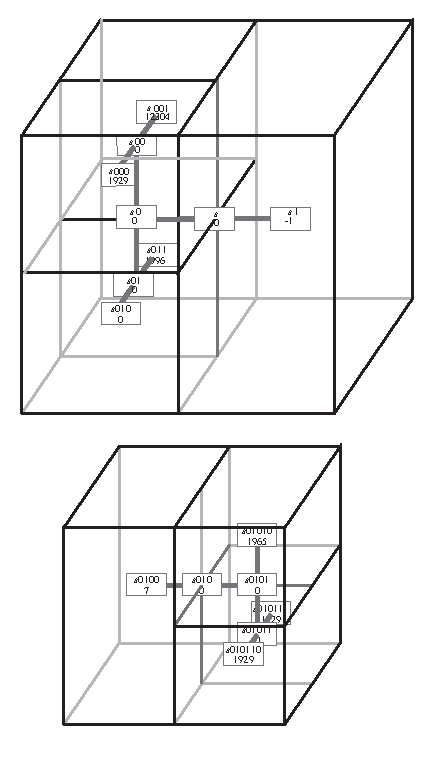
\includegraphics[scale=1.250]{fig5.1}

	\caption{
		Six levels of subdivision, in two projections,
		with all the trimmings.
	}
\end{figure}

$Z(s1)$ is ignored, so the checker would indicate this omission
in its report.  In fact, $Z(s1)$ is one of the 11 exceptional sub-boxes (seven boxes after joining abutters), specifically
$X_{5a},$ hence killed automatically.

The use of condition ``L(w)'' so deep in the tree is unusual.
In this case, it is because the manifold in the exceptional sub-box
has ${\textrm length}(f) = {\textrm length}(w)$, so that the program will frequently
come to places where it can bound ${\textrm length}(f) > {\textrm length}(w)$ nearby.

The sequence $\ 0, 1929, 1929\ $ in the 
input for $Z(s)$ tells the checker to
subdivide $Z(s01011)$, and then use the condition 1929
on both halves to kill   them separately, 
thereby killing $Z(s01011)$.
As mentioned above,
the reason for carrying out this  subdivision 
is that the remainder/error bound in the calculation
 for $Z(s01011)$ using condition 1929 was not good enough
to prove that the sub-box is killed directly. 
 
 


In the input for $Z(s)$ we could have
replaced 
 $\ 0, 1929, 1929\ $ with 1929 alone
and then the checker
program itself would be smart enough to carry out
the subdivision after 1929 failed to kill the sub-box
$Z(s01011).$
This recursive subdivision tool is quite useful when dealing with the 
remainder/error term---if a killerword barely misses killing off a sub-box, then recursively subdivide the sub-box and
use the same killerword on the pieces until it succeeds.   We note that the theoretical error arising from using a
first-order Taylor approximation is likely to be significantly improved by subdivision, whereas the
round-off error is relatively unaffected because the killerword
used is unchanged (hence the number of mathematical operations
performed is unchanged).

The binary numbers used by the computer require too much space to print.
In the example calculation which follows, we instead use decimal 
representations (although we print fewer digits than could
be gotten from the 53 binary digits used for the actual calculations).

The sub-box $Z(s01011)$ is the region where 
$$\left(\begin{array}{c} 
-1.381589027741\ldots  \le  {\mathrm Re}(L')  \le  -1.379848991182\ldots\cr
-1.378124546093\ldots  \le  {\mathrm Re}(D')  \le  -1.376574349753\ldots\cr
0.999893182771\ldots  \le {\mathrm Re}(R')  \le  1.001274250703\ldots\cr
-2.535837191243\ldots  \le  {\mathrm Im}(L')  \le  -2.534606799593\ldots\cr
\phantom{-}2.535404997792\ldots  \le  {\mathrm Im}(D')  \le  -2.534308843448\ldots\cr
-0.001953125000\ldots  \le  {\mathrm Im}(R')  \le  0.000000000000\ldots\phantom{-}\cr
\end{array}\right)$$


At this point, we would like to compute $$f,\ w,\ g = f^{-1}wf^{-1}w^{-1}f^{-1}w^{-1}fw^{-1}f^{-1}w^{-1}f^{-1}wf^{-1}wfww, \ {\textrm length}(g),$$ 
\noindent 
and so on.  
However, these items take on values over an entire sub-box and thus are computed via AffApproxes (first-order Taylor
approximations with remainder/error bounds), which are not formally defined until the next section.  We
complete
Example \ref{GMT 5.4}
 at the end of 
	Chapter (CHECKTHIS: FIXME(6)).  %TODO: chxref
\end{example}

\vglue9pt 
\begin{remark} \label{GMT 5.5}
.  For those planning on looking at the program {\textit verify}
we now tie in the above description of its workings to a portion of the actual code in the program.  We note that the CWeb version of {\textit verify} is extensively documented, and is organized so that the most important details are presented first.

If the executable version of {\textit verify} is called {\textit verify} and we are in the correct place with respect to the location of the data, then a typical UNIX command line would be 
$$
\hbox{\texttt zcat data/000000.gz | verify 000000 > output000000} 
$$
This would run {\textit verify} at the node 000000, and, when needed, would pipe in the unzipped data from \hbox{\texttt
data/000000.gz}.  This unzipped data contains the tree decomposition of the parameter space at the sub-box 000000. 
The output from {\textit verify} would be redirected to the file \hbox{\texttt output000000}.

In {\textit verify}, \hbox{\texttt main} would check for syntax errors in the command line, and if there were no such errors, would read the location 000000 into the character array \hbox{\texttt where}  and compute that the \hbox{\texttt depth} of \hbox{\texttt where} was 6, which means that 000000 contains
six subdivisions.   It would then immediately print 
$$
\hbox{\texttt verified 000000 - } \{$$
into the file \hbox{\texttt output000000}, and then call the function {\textit verify}, as follows:
$$
\hbox{\texttt verify(where, depth, 0);}
$$

The function \hbox{\texttt verify(where, depth, autocode)} is now invoked; this time with \hbox{\texttt autocode} equal to 0.  {\textit Verify} would first check that \hbox{\texttt depth} was not too deep.  Next, {\textit verify} checks if \hbox{\texttt autocode} is equal to 0, which it is, so it reads in the next (in this case, the first) integer from the unzipped file \hbox{\texttt data/000000.gz}, and sets \hbox{\texttt code} equal to this integer.  Now, {\textit verify} recursively calls itself on the left child (0000000) of the \hbox{\texttt where} box and the right child (0000001) of the
 \hbox{\texttt where} box:
\begin{eqnarray*}
\noalign{\vskip-12pt}
&&
\hbox{\texttt where[depth] = \hbox{`}0\hbox{'};}
\\
&& \hbox{\texttt verify(where, depth + 1, code);}
\\
&&
\hbox{\texttt where[depth] = \hbox{`}1\hbox{'};}
\\
&&\hbox{\texttt verify(where, depth + 1, code);}
\end{eqnarray*}
In general, \hbox{\texttt verify(where, depth, autocode)} does the following.  It checks to see that \hbox{\texttt depth} is not too deep.  Then if \hbox{\texttt autocode} is equal to 0, it recursively calls itself on its left and right children.  If \hbox{\texttt autocode} is not equal to 0, then \hbox{\texttt code} is set equal to \hbox{\texttt autocode}, and
three possibilities can occur.  Either, 
\vglue9pt
1)  \hbox{\texttt code} is less than zero, in which case we are at 
a sub-box to be skipped, 
 and {\textit verify} prints out its location  (\hbox{\texttt where}) in \hbox{\texttt output000000} and recursively moves on to the next node in the tree, or 
\vglue9pt
2) \hbox{\texttt code} is greater than zero and it invokes a condition/killerword from the file {\textit conditionlist} which kills the entire sub-box \hbox{\texttt where}
in which case \hbox{\texttt verify} simply recursively moves on to the next node in the tree, or 
\vglue9pt
3) \hbox{\texttt code} is greater than zero and it invokes a condition/killerword from the file {\textit conditionlist} which does not kill the entire sub-box \hbox{\texttt where}, in which case
\hbox{\texttt verify} subdivides the sub-box \hbox{\texttt where} and recursively calls itself on the left child and the right child, using the same \hbox{\texttt code}:
\begin{eqnarray*}
&&\hbox{\texttt where[depth] = \hbox{`}0\hbox{'};}
\\ &&\hbox{\texttt verify(where, depth + 1, code);}
\\ &&\hbox{\texttt where[depth] =\hbox{`}1\hbox{'};}
\\ &&\hbox{\texttt verify(where, depth + 1, code);}
\end{eqnarray*}
In this way {\textit verify} tests the entire starting box, in this case the sub-box 000000, and if successful at killing
it minus the omissions which it prints out, it finishes \hbox{\texttt main} by printing out a right bracket into \hbox{\texttt output000000}. \end{remark}
  
